\documentclass[conference]{IEEEtran}
\IEEEoverridecommandlockouts

% Packages
\usepackage{cite}
\usepackage{amsmath,amsfonts}
\usepackage{algorithm}
\usepackage{algpseudocode}
\usepackage{graphicx}
\usepackage{textcomp}
\usepackage{xcolor}
\usepackage{booktabs}
\usepackage{adjustbox}
\usepackage{listings}

\usepackage{verbatim}
\usepackage{multirow}

\def\BibTeX{{\rm B\kern-.05em{\sc i\kern-.025em b}\kern-.08em
    T\kern-.1667em\lower.7ex\hbox{E}\kern-.125emX}}

\begin{document}

\title{Deliverable report \\
\footnotesize \textit{"Vittorio Polci": Mat: 257817, \texttt{vittorio.polci@unitn.it}, GitRepo: \texttt{https://github.com/vittorio01/GPU-Computing-2025-257817}}}

\maketitle

\begin{abstract}
This deliverable discusses about the implementation of different parallel solutions of the SpVM algorithm between CSR matrices and a general vector,
with a final benchmark that compares all solution toghether. 

\end{abstract}

\begin{IEEEkeywords}
Sparse Matrix, SpMV, CUDA, Parallelization, Storage Format
\end{IEEEkeywords}

\section{Introduction}
The algorithm of sparse matrix-dense vector multiplication (SpMV) is an optimized version of the traditional matrix-vector multiplication
designed to handle cases where the matrix is organized in a low density of non-zero entries. 
This technique is particularly useful in scenarios that involves very large sparse matrices because it allows to reduce the used space for 
storing that large structures and, at the same time, optimizes memory access patterns during computational steps. 

Because the SpMV multiplication should handle matrices with millions or billions of not null elements, to obtain good results is necessary to use parallelization techniques 
on GPUs rather than sequential solution for CPUs. 

\section{Problem Statement}
In the SpVM multiplication we consider a matrix coded in a sparse format (in this case the CSR format) and an input vector that has the same size of its columns number. 

Each elements of the resulting vector is computed by performing the dot products of each not null elements of the matrix with the input vector and accumulating them in the corresponding row position.
At this point the main objectives are:
\begin{enumerate}
    \item Create a first sequential algorithm that performs the same operation on a sparse CSR matrix.
    \item Parallelize the first CPU implementation with CUDA and compare them in terms of performances and resurces utilization. 
\end{enumerate}

\subsection{Storage Format}
The CSR for sparse matrices is a storage format that involves three different arrays to represent the information: 
\begin{itemize}
    \item The data array, that contains all not null terms of the original matrix.
    \item The column array, where for each element in the data vector specifies its column coordinate.
    \item The row array, which contains the start and the end pointers for each row to the data and column arrays. these two pair of pointers indicates which nut null terms in the data array are contained in that specific row. 
\end{itemize}
The size of the data and column arrays depends on the number of not null elements and the size of the row array depends on the number of the rows in the original matrix. 
\begin{figure}[H]
    \centering
    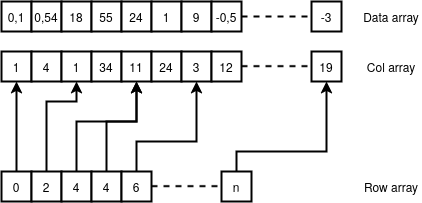
\includegraphics[width=0.8\linewidth]{images/CSR.png}
    \caption{Data organization in CSR structure}
    \label{fig:csr-format}
\end{figure}

\subsection{Parallelization}
To improve the overall performance, the parallel implementations of the first algorithm are designed to be executed on Nvidia GPUs and programmed in CUDA.
The CUDA language model permits to run a kernel on different concurrent threads, which are scheduled and executed by computational elements called CUDA cores. 

To improve the performance and the organization of the parallel algorithms, CUDA architectures provides:
\begin{itemize}
    \item {\it{Warp organization}}, where groups of 32 threads can synchronize and dhare data using predefined function for reductions.
    \item {\it{Block organization}}, where more warps can syncronize themself using atomic operations, barriers and shared memory.
    \item {\it{Shared memory}}, which is divided in more blocks and used to improve data reusage, optimize the global memory transfers and other purposes. 
    \item {\it{Read only cache}}, which is a L1 read only cache that can be assigned by the programmer for improving data transfer for casual and repetitive accesses. 
\end{itemize}

\section{State of the Art}
There already are multiple c++ libraries that performs CSR SpMV multiplications like:
\begin{itemize}
    \item cuSPARSE\cite{cuSPARSE}, the official library supported by Nvidia that can perform multiplication between matrices and vectors in different formats with CUDA. 
    \item Ginkgo\cite{ginkgo}, like MAGMA offers high-performance solution for multicore linear algebra algorithms for different platforms.
\end{itemize}
\section{Methodology and Contributions}\label{sec:methodology}

\subsection{Dynamic algorithm}
To reduce the unbalance 
\begin{enumerate}
    \item The row array is splitted in equal subsection for different blocks using again the ceiling division. 
    \item For each block a variable in the shared memory $pendingRow$ is initialized and used to contain the next row number that is waiting for the assignment. 
    \item Each thread uses the function $atomicAdd(pendingRow,1)$ to increment the value of $pendingRow$ and, at the same time, read its content
    \item Using the value obtained each thread computes the products and the accumulation of the entire row and repeats step 3 and 4 until the block reach the end of its subsection. 
\end{enumerate}

\begin{algorithm}[h!]
\caption{Dynamic SpVM algorithm}
\algorithmicrequire~input, output and matrix structures.
\begin{algorithmic}[1]
\Procedure{vmcsrMul}{$output$, $matrix$, $input$}
\State $blockStart,blockEnd$ \Comment{Ceiling division}
\State $pendingRow=0$ \Comment(only thread 0);
\State $syncthreads()$
\While {${true}$}
\State $pendingRow=atomicAdd(pendingRow,1)$
\State $+blockStart$
\If {$pendingRow>blockEnd$} \Return \EndIf
\State $startRow=matrix.rowArray[pendingRow]$
\State $endRow=matrix.rowArray[pendingRow+1]$
\State $acc=0$
\While{${startRow<endRow}$}
\State $col=matrix.colArray[startRow]$
\State $acc+=$
\State $matrix.dataArray[startRow]$
\State $\ \ *input.dataArray[col]$
\State $startRow++$
\EndWhile
\State $output.dataArray[pendingRow]=acc$
\EndWhile
\EndProcedure
\end{algorithmic}
\label{alg:dynamic1}
\end{algorithm}

This dynamic assignment for threads in the same block implemented in the algorithm \ref{alg:parallel2} tries to mitigate the unbalanced workload introduced in some rows. 
In facts, if some thread spend too much time when computing a single row, other available threads may perform also rows that in a static division should be reserved for others.  

\subsection{Optimized Dynamic algorithm}
The dynamic algorithm can be improved further using a better organization of workload between threads. More performance can then be obtained by:
\begin{itemize}
    \item Dividing the workload between blocks using an approach based on the number of not null elements instead the rows. To achieve this, the ceiling division can be performed on the not null array instead on the row array and a binary search can be performed to find the relative rows boundaries. 
    \item Assigning a warp for each row instead a single thread. In this way, because 32 threads are assigned per row, longer rows can be processed in shorter time and the partials obtained by threads in the same row can be reduced using more {$\_\_shfl\_down\_sync$} functions.
    \item Assigning the read only cache on the input vector to improve the speed of the algorithm by leveraging on the data reusage.
\end{itemize}

\begin{algorithm}[h!]
\caption{Kernel used for the preliminar block division. The kernel is launched with the same number of blocks of the main kernel \ref{alg:dynamic2} but only one thread per block.}
\algorithmicrequire~ matrix structure and the preinitialized blockDivision array on the GPU's global memory.
\begin{algorithmic}[1]
\Procedure{vmcsrDiv}{$matrix$, $blockDivision$}
\State $blockStart,blockEnd$ \Comment{Ceiling division on the not null element's array}
\State \text{\dots}\Comment{output vector initialization phase}
\If{$blockIdx.x==0$}
\State $blockDivision[0]=0$
\State $blockSivision[blockDim.x-1]=rowSize$
\State $\textbf{return}$
\EndIf
\State $row=-1$
\State $left=0$
\State $right=rowSize$
\While{$left<=right$}
\State $mid=(left+right)/2$
\If{rowArray[mid]<=blockStart}
\State $row=mid$
\State $left=mid+1$
\Else 
\State $right=mid-1$
\EndIf
\EndWhile
\State $blockDivision[blockIdx.x]=row$
\EndProcedure
\end{algorithmic}
\label{alg:binary_search}
\end{algorithm}

\begin{algorithm}[h!]
\caption{Optimized dynamic algorithm}
\algorithmicrequire~matrix structure, block division array, input vector and output vector structures.
\begin{algorithmic}[1]
\Procedure{vmcsrMul}{$output$, $matrix$, $input$, $blockDivision$}
\State $blockStart=blockDivision[blockIdx.x]$
\State $blockEnd=blockDivision[blockIdx.x+1]$
\State $pendingRow=0$ \Comment(only thread 0);
\State $syncthreads()$
\State $row=\underline{Row Election}$ 
\While {$row<blockEnd$}
\State $startRow=matrix.rowArray[row]$
\State $endRow=matrix.rowArray[row+1]$
\State $acc=0$
\While{${startRow<endRow}$}
\State $idx=min(startRow+laneId,endRow)$
\State $col=matrix.colArray[idx]$
\State $acc+=$
\State $(matrix.dataArray[idx]$
\State $\ *\_\_ldg(input.dataArray[col]))$
\State $\ *(startRow+laneId<endRow)$
\State $startRow++$
\EndWhile
\State $acc=\underline{ReduceSum}$
\If {$laneId==0$}
\State $output.dataArray[row]=acc$
\EndIf
\State $row=\underline{Row Election}$ 
\EndWhile
\EndProcedure
\end{algorithmic}
\label{alg:dynamic2}
\end{algorithm}

\begin{algorithm}[h!]
\caption{Row election System}
\begin{algorithmic}[1]
\Procedure{RowElection}{}
\If {$laneId==0$}
\State $row=atomicAdd(pendingRow,1)$
\State $\ +blockStart$
\EndIf
\State $\_\_shfl\_sync(0xffffffff,row,0)$
\EndProcedure
\end{algorithmic}
\label{alg:rowElection}
\end{algorithm}


\begin{algorithm}[h!]
\caption{Warp reduction system}
\begin{algorithmic}[1]
\Procedure{reduceSum}{acc}
\State $acc=\_\_shfl\_down\_sync(0xffffffff,acc,16)$
\State $acc=\_\_shfl\_down\_sync(0xffffffff,acc,8)$
\State $acc=\_\_shfl\_down\_sync(0xffffffff,acc,4)$
\State $acc=\_\_shfl\_down\_sync(0xffffffff,acc,2)$
\State $acc=\_\_shfl\_down\_sync(0xffffffff,acc,1)$
\EndProcedure
\end{algorithmic}
\label{alg:reduceSum}
\end{algorithm}

\subsection{Shared cooperative algorithm}
The algorithm \ref{alg:dynamic2} does not adds a significant improvement for heavily unbalanced matrices. Another approach that tries to handle also those cases uses the shared memory to contain three different buffers:
\begin{itemize}
    \item {\it{sharedBuffer}}, a space used as buffer to contain the result of the multiplication between elements of the matrix and the input vector (each thread operates on around 14 elements).
    \item {\it{loadedRows}}, a space of {$blockSize.x$} cells used as cache for parts of the CSR row vector (each threads loads one pointer).
    \item {\it{rowsBuffer}}, a space of {$blockSize.x-1$} used for accumulating partials for a small amount of rows (almost each thread maintaines one cell). 
\end{itemize}
Using these three different shared spaces, each block performs these steps:
\begin{enumerate}
    \item The entire block cooperates to prepare the shared memory for processing {$blockSize-1$} rows by initializing with zeroes the {\it{rowsBuffer}} space and loading the necessary CSR pointers from the row array in the {\it{loadedRows}} space.
    \item All threads load a certain amount of the required elements from the matrix and the input vector in a fully coaleshed way, perform the products and save the result in {\it{sharedBuffer}}.
    \item The loaded elements are divided then in equal strides strides and the threads perform binary searches on the {\it{loadedRows}} space to identify the correspondent rows of the first elements of the strides. Then the strides are reduced in partials and accumulated in the {\it{rowsBuffer}} using $atomicAdd()$.
            In this phase, a thread can eventually operate in multiple rows.
    \item The step 2 and 3 are performed until all not null elements of all rows' subset are processed.
    \item Each threads stores one result from the {\it{rowsBuffer}} to the output vector in the global memory.
    \item All steps from 1 to 5 are repeated until all rows of the matrix are processed. 
\end{enumerate}
The procedure \ref{alg:shared1} shows a heavily simplified representation of the shared cooperative algorithm.
\begin{algorithm}[h!]
\caption{Shared cooperative algorithm}
\algorithmicrequire~matrix structure, block division array, input vector and output vector structures.
\begin{algorithmic}[1]
\Procedure{vmcsrMul}{$output$, $matrix$, $input$, $blockDivision$}
\State $blockStart, blockEnd$ \Comment(From binary search kernel).
\State $sharedBuffer, rowsBuffer, loadedRows$
\For{$(blockDim.x-1)\ \text{steps}\ \textbf{in} [blockStart,blockEnd]$}
\If{$threadIdx.x\ \textbf{in}\ rows\ block$}
\State {\underline{Row space initialization}}
\EndIf
\For {$sharedBufferDim\ \text{steps}\ \textbf{in}\ \it{blockNotNulls}$}
\State \underline{cooperative multiplication on shared buffer}
\State \underline{Stride division of shared Buffer}
\State \underline{Binary search of first lane element}
\State \underline{Stride reduction}
\EndFor
\If{$threadIdx.x\ \textbf{in}\ rows\ block$}
\State {\underline{Rows unloading to global}}
\EndIf
\EndFor
\EndProcedure
\end{algorithmic}
\label{alg:shared1}
\end{algorithm}

\section{System Description and Experimental Set-up}
\subsection{Dataset description}
A dataset composed by 6 matrices is used for testing and benchmark all four algorithms. These matrices containes a number of not null elements between 1 and 1,5 million of not null elements and they have different organization of the elements and dispersion that challenges the algorithms in different ways:
The used dataset is obtained from the SuiteSparse Matrix Collection \cite{suitesparse}, a website that contains sample matrices which can be used for benchmarking algorithms. 

\begin{table}[h]
    \centering
    \begin{adjustbox}{width=\columnwidth}
    \begin{tabular}{llllrl}
    \toprule
    \textbf{Dataset} & \textbf{Dimension (R x C)} & \textbf{Non-zero entries} & \textbf{Type} \\
    \midrule
    dbir2 \cite{dbir2} & 18,906 x 45,887 & 1,158,159 & Unbalanced rows \\
    ex11 \cite{ex11} & 16,614 x 16,614 & 1,096,948  & Diagonally distributed (low density) \\
    language \cite{language} & 399,130 x 199,130 & 1,216,334 & Upper triangular \\
    Linux\_call\_graph \cite{linuxcallgraph} & 324,085 x 324,085 & 1,208,908 & Dense matrix (worst case) \\
    nemeth24 \cite{nemeth24} & 9,506 x 9,506 & 1,506,550 & Diagonally distributed (best case) \\
    twotone \cite{twotone} & 120,750 x 120,750 & 1,206,265 & Diagonally distributed (moderate dispersion) \\
    \bottomrule
    \end{tabular}
    \end{adjustbox}
    \vspace{1em}
    \caption{Structural patterns of the benchmark sparse matrices.}
    \label{tab:my_label}
\end{table}

\subsection{System Description}
The system used for the execution of the benchmarks is uses CUDA 12.3.2, GCC 11.5.0, and is composed by a Intel(R) Xeon(R) Silver 4214 CPU and A Nvidia A30 GPU.  

\begin{table}[h]
    \centering
    \begin{adjustbox}{width=0.8\columnwidth}
    \begin{tabular}{lll}
    \toprule
    \textbf{Characteristic} & \textbf{Value} & \textbf{Device}\\
    \midrule
    Global memory & 24 GB &  \multirow{5}{*}{\textbf{GPU: Nvidia A30}} \\
    Theoretical BW & 933 GB/s \\
    CUDA Cores & 10752 \\
    SM Number & 108 \\
    FP32 Performance & 10.3 TFLOPS \\
    \midrule 
    Cores number & 12 & \multirow{3}{*}{\textbf{CPU: Intel(R) Xeon(R) Silver 4214}} \\
    Threads number & 24 \\
    Clock speed & 2.2Ghz \\
    \bottomrule
    \end{tabular}
    \end{adjustbox}
    \vspace{1em}
    \caption{Benchmark system specs}
    \label{tab:benchmarkSystem}
\end{table}

\subsection{Experimental Set-up}
The performance is measured using the execution time elapsed measured with $cudaEventRecord$ functions for CUDA algorithms. 
\subsection{Block size estimation}
The parameters used for launching the kernels are calculated empirically in base of the amount of shared memory available per block, the number of cuda cores per SM and the size of the input matrix. In particular:
\begin{itemize}
    \item The number of threads per block is equal to the number of CUDA cores per SM divided by the available shared memory per block in MB ($cores/sharedPerSM$).
    \item The number of blocks is equal to the number of not null elements of the input matrix divided by a constant obtained empirically of around 3328 ($notNull/NotNullPerBlock$).
    \item In the kernel \ref{alg:shared1}, the dimension of the shared memory is related on the number of elements that each thread should load in the {\it{sharedBuffer}} (the best performances are obtain for 14 elements per tread).
\end{itemize}
\section{Experimental Benchmarks}
The following tables shows the values of GFLOPs/s (\ref{tab:GFLOPS}) and effective bandwidth (\ref{tab:BW}) obtained from benchmarking on 256 blocks of 512 using float values. 
The figure \ref{fig:flops-graph} gives also a visualization of table \ref{tab:GFLOPS}.
\begin{table}[h]
    \centering
    \begin{adjustbox}{width=0.8\columnwidth}
    \begin{tabular}{lllll}
    \toprule
    \textbf{Matrix} & \textbf{Parallel 1} & \textbf{Parallel 2} & \textbf{Parallel 3} & \textbf{Sequential} \\
    \midrule
    dbir2 \cite{dbir2} & \textbf{152,93} & 142,78 & 34,8 & 1,69 \\
    ex11 \cite{ex11} & 71,44 & \textbf{71,74} & 21,02 & 0,38 \\
    language \cite{language} & 31 & \textbf{82,4} & 1,91 & 0,32\\
    Linux\_call\_graph \cite{linuxcallgraph} & 0,85 & 1,72 & \textbf{2,51} & 0,25 \\ 
    nemeth24 \cite{nemeth24} & 43,4 & \textbf{50} & 16,81 & 0,37 \\
    twotone \cite{twotone} & 44,42 & \textbf{51,84} & 4,7 & 0,42 \\
    \bottomrule
    \end{tabular}
    \end{adjustbox}
    \vspace{1em}
    \caption{GFLOPs/s comparison between parallel and sequential implementations}
    \label{tab:GFLOPS}
\end{table}
\begin{table}[h]
    \centering
    \begin{adjustbox}{width=0.79\columnwidth}
    \begin{tabular}{lllll}
    \toprule
    \textbf{Matrix} & \textbf{Parallel 1} & \textbf{Parallel 2} & \textbf{Parallel 3} \\
    \midrule
    dbir2 \cite{dbir2} & \textbf{932,56} & 870,66 & 212,49 \\
    ex11 \cite{ex11} & 435,15 & \textbf{437} & 128,03  \\
    language \cite{language} & 250,37 & \textbf{656,65} & 15,27 \\
    Linux\_call\_graph \cite{linuxcallgraph}& 6,52 & 13,11 & \textbf{19,12} \\ 
    nemeth24 \cite{nemeth24} & 263,8 & \textbf{305,51} & 102,18  \\
    twotone \cite{twotone}& 292,8 & \textbf{241,75} & 31,03  \\
    \bottomrule
    \end{tabular}
    \end{adjustbox}
    \vspace{1em}
    \caption{Bandwidth (GB/s) comparison between parallel implementations}
    \label{tab:BW}
\end{table}
\begin{figure}[H]
    \centering
    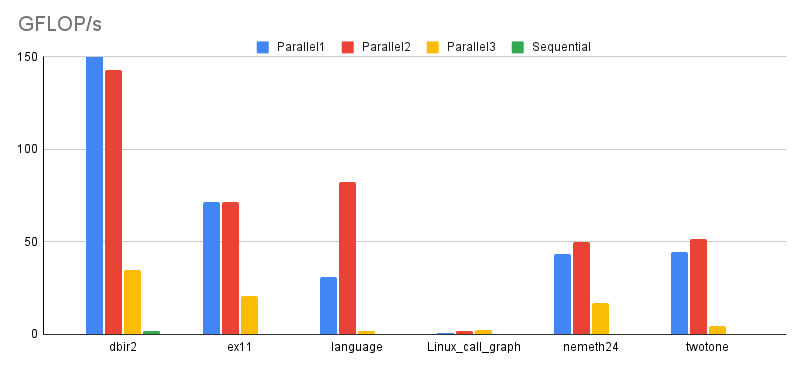
\includegraphics[width=1\linewidth]{images/GFLOP_s.png}
    \caption{Performance offerences between the four algorithms}
    \label{fig:flops-graph}
\end{figure}

\section{Results and conclusion}
The results indicates that:
\begin{itemize}
    \item The best situation is when the not null elements in the matrix are concentrated on the diagonal.
    \item If the number of not null elements per row is almost uniform for each row in the matrix, the first and the second parallel algorithms give similar results. 
    \item The second parallel algorithm behaves better in different situations than the others implementations thanks to its load distribution system.
    \item The third parallel algorithm is more performant that the others only if the number of not null elements per row is very large and the dispersion of the matrix is high.
\end{itemize}
Also the block size affects the performances of the algorithms. In facts:
\begin{itemize}
    \item In the first implementation the block size does not affect much the performances because the static allocation of workload. 
    \item In the second implementation a lower block size may reduce the concurrency on the assignment system of the rows. 
    \item In the third implementation a block size that is much lower that the average number of not null elements per row is more convenient because reduces significantly the concurrency introducted when accumulating the result on the output vector. 
\end{itemize}
\bibliographystyle{IEEEtran}
\bibliography{references}

\end{document}

